\clearpage
\newpage

\subsubsection{Estensione E: Errore Durante la Modifica dello Stato delle Categorie di Notifica}

Nel caso in cui si verifichi un errore durante il tentativo di modifica dello stato di una categoria di notifica, viene visualizzato un messaggio di errore sotto forma di un popup informativo. Il messaggio informa l'utente che la modifica non è riuscita e lo invita a riprovare più tardi, senza salvare le modifiche effettuate.

\vspace{0.5cm}
\subsubsection{Gestione dell'Errore e Feedback Utente} Il popup di errore presenta i seguenti elementi chiave: \begin{itemize} \item \textbf{Messaggio chiaro e informativo}: il messaggio comunica all'utente che l'operazione non è andata a buon fine, senza entrare in dettagli tecnici, per ridurre il rischio di frustrazione. L'utente viene anche informato che l'operazione non è stata completata e che le modifiche non sono state salvate. \item \textbf{Pulsante “Ok”}: consente all'utente di chiudere il popup e tornare all'interfaccia principale. Il pulsante di conferma è chiaro e consente di riprendere l'interazione senza indugi. \end{itemize}

\subsubsection{Principi di Design Applicati} L'approccio di gestione dell'errore in questa estensione si fonda sui seguenti principi di UX e usabilità: \begin{itemize} \item \textbf{Visibilità dello stato del sistema} \cite{nielsen1995}: l'errore è comunicato all'utente attraverso un popup che evidenzia chiaramente che il sistema non è riuscito a completare l'operazione. \item \textbf{Prevenzione degli errori} \cite{nielsen1995}: sebbene l'errore non possa essere evitato completamente, il sistema offre un feedback immediato e comprensibile, impedendo all'utente di rimanere confuso o incerto sullo stato dell'operazione. \item \textbf{Semplicità e chiarezza} \cite{nielsen1995}: il messaggio di errore è semplice e diretto, senza sovraccaricare l'utente con informazioni tecniche. L'invito a riprovare più tardi mantiene il flusso di lavoro semplice e lineare. \item \textbf{Controllo dell'utente} \cite{norman1988}: l'utente ha il pieno controllo sulla gestione dell'errore, poiché il popup permette di chiudere facilmente l'interfaccia e riprendere l'attività, mantenendo un'esperienza utente fluida. \end{itemize}

Questa soluzione di gestione dell'errore è progettata per garantire un'esperienza utente chiara e senza frustrazioni, minimizzando il disagio derivante da errori tecnici imprevisti e offrendo un percorso semplice per riprendere l'interazione.
\begin{figure}[ht]
    \centering
    \begin{tikzpicture}[node distance=1.5cm and 1cm, auto]
        % Nodo per immagine 1 con didascalia sotto
        \node (img1) {
            \begin{tabular}{c}
                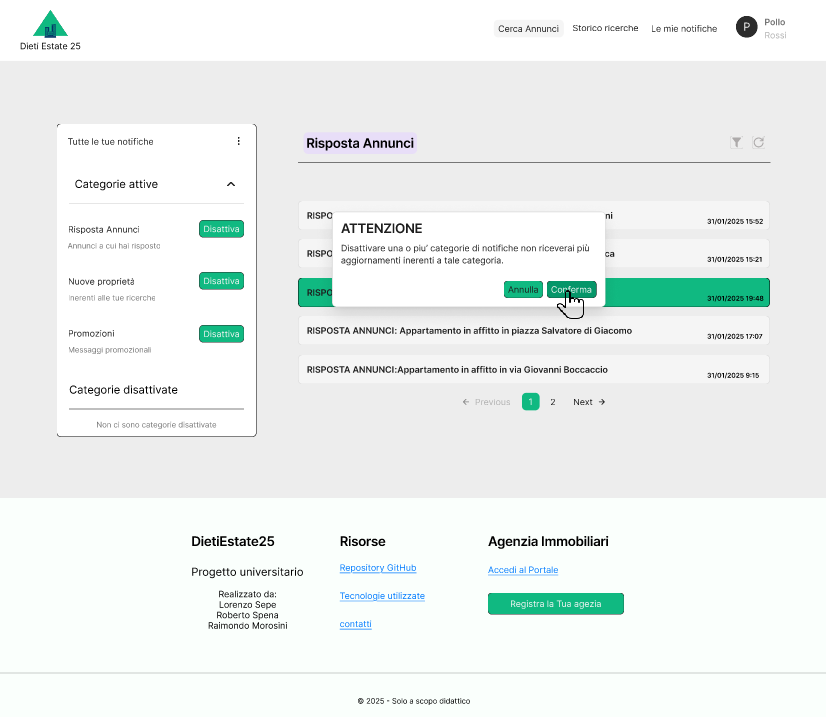
\includegraphics[width=0.6\textwidth]{Immagini/Mockup/notifiche/estensione E/click conferma.png} \\
                Cockburn: step 7
            \end{tabular}
        };
        
        % Nodo per immagine 2 con didascalia sotto, posizionato a destra di img1
        \node (img2) [below=of img1] {
            \begin{tabular}{c}
                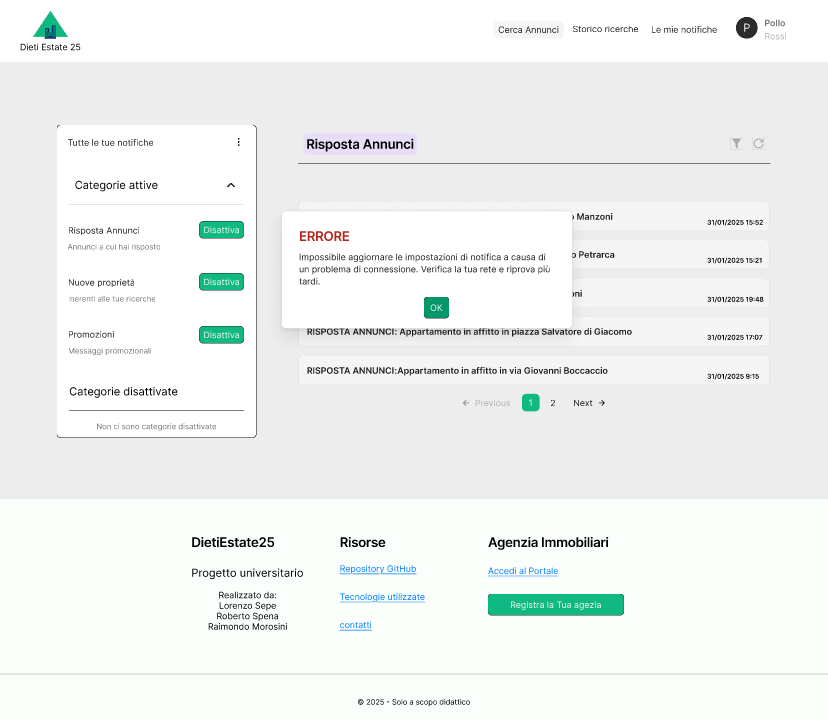
\includegraphics[width=0.6\textwidth]{Immagini/Mockup/notifiche/estensione E/errore.png} \\
                Cockburn: Extension E.7/E.8
            \end{tabular}
        };
        
        % Disegna le frecce
        \draw[->, thick] (img1) -- (img2);
      
    \end{tikzpicture}
    \caption{Mockup: estensione E della tabella di Cockburn del caso d'uso disattiva/attiva categoria notifica}
    \label{fig:mockup_estensione_E_disattiva_notifiche}
\end{figure}

\newpage

